\documentclass{article}
\usepackage[final]{nips_2017}
\usepackage[utf8]{inputenc} % allow utf-8 input
\usepackage[T1]{fontenc}    % use 8-bit T1 fonts
\usepackage{hyperref}       % hyperlinks
\usepackage{url}            % simple URL typesetting
\usepackage{booktabs}       % professional-quality tables
\usepackage{amsfonts}       % blackboard math symbols
\usepackage{nicefrac}       % compact symbols for 1/2, etc.
\usepackage{microtype}      % microtypography
\usepackage{graphicx}
\usepackage{wrapfig}
\title{Family kinship Recognition Using Deep Learning}

\author{
  Bruce Jianye Liu\\
  Department of Computer Science\\
  Stanford University\\
  \texttt{bruceliu@stanford.edu} \\
}


\begin{document}
% \nipsfinalcopy is no longer used

\begin{center}

\includegraphics[width=3cm, height=0.7cm]{CS230}
\end{center}

\maketitle

\section{Problem Description}
Half of genetic information is passed down from parents to children. Therefore
people biologically related share delicate similiarities. This declicacy could
be easily caught by human eyes, looking at family photos. While computer vision
performance improving during the past decade, it becomes possible to use
meachine learning to capture the different. Computer vision based kinship
recognition could lead variety of usefull applications in reality such as
missing-children parents matching, family album organization, socal networking
apps, lost sibling/relatives searching, crime investigation. In this paper, we
propose a fine-tuned KinNet model to identify the relationship between two
faces -- parent-children, sibling-sibling, none-kinship, and same person. We
achieved 70 percent accuracy.

Solely relying on face pairs for kinship verification might be hard to achieve
higher accuracy since people without any family relation would look simliar to
each other. There are other metrics that we could consider to determine if the
kinship exists. Such information includes hands shape, nail types, foot toes,
ears, hairs. Due to time limitation and team size, we aren't able to collect
this data. Otherwise the prediction would improve a lot.

\section{Related Works}

Even thought many researcher have tried traditional approach to on image
recogintion tasks, Deep learning shows state-of-art achievement out-perform
other method by two order in computer image tasks. One of well-known image
recognition tasks is ImageNet[5] classification, which contains 14
million images labeled to roughly 22,000 catergories, and is widely used in
literacy as a large visual database for visual object recognition.

Starting from 2009, many neural network models are designed by researchers,
among them AlexNet[6] from University of Toronto in 2012, GoogLeNet
(Inception)[7] from Google in 2014, VGG[8] from Oxford Vision Geometry Group in
2015, and ResNet[9] form Microsoft Research showing significant impact on
academia. The error rate reached as low as 3.57\% surpassing human performance.

Beside Imagenet dataset, Labeled Faces in the Wild (LFW)[10] dataset and
Youtube Faces DB are widely used in face recognition tasks. Despite many other non-deep learning models have good performance, deep neural network models keep top records on this task, such as faceNet[2] designed by Schroff etc. achieved 99.63\% accuracy.

Similar to face verification problem, kinship recognition is another task that
attracts many researchers to put effect on.  Past kin recognition work mainly
focus on kinship verification, to decide whether two faces have kinship, family
classification, classifing a face to a family, and family member regcontion,
determining 2 faces siblings or parents. Over the past decades, many methods
has been proposed on this research, including hand-crafted feature, face
ecnodings, and metric learning[3].

\section{Dataset}

\begin{wrapfigure}{l}{0.25\textwidth}
\caption{108x124 face sample}
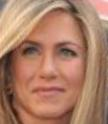
\includegraphics{img/P00241_face0}
\end{wrapfigure}

We are going to use Families In The Wild (FIW) Database[1]. FIW is the largest
and most comprehensive database available for kinship recognition. We use
version 0.1.2 at writing time, which include 13,188 faces from 1018 families.
Event though it has 11 kinship types, father-daughter (F-D), father-son (F-S),
mother-daughter (M-D), mother-son (M-S), brother-brother (B-B), sister-sister
(S-S), grandfather-granddaughter (GF-GD), grandfather-grandson (GF-GS),
grandmother-granddaughter (GM-GD), grandmother-grandson (GM-GS), to our study,
siblings and parent-child types are what we are going to use. Adding up 64669
F-D, 46143 F-S, 68935 M-D, 48940 M-S types, we get 22687 parent-child photos
while sibling types contains 55937 photos. All face images are 108*124*3 size.
The same face data is generated by selecting pictures with the same FaceID.
Non-related picture pairs are generated with pictures in the Family folder and
one of the faces in the family.

\begin{table}[h]
	\centering
	\begin{tabular}{ | c || r r | }
		\hline
		\multicolumn{3}{|c|}{face-pair image distribution} \\
		\hline
		pair types&face-pair number&percentage\\
		\hline
			parent-child & 228,687 &21.17\% \\
			siblings & 55,937 & 5.18\% \\
			same & 230,938 & 21.38\% \\
			unrelated & 564,496 & 52.27\% \\
		\hline
			& 1,080,058 & \\
		\hline
	\end{tabular}
	\caption{Training data distribution}
	\label{table:1}
\end{table}

Table 1 distrubtion may affect our model less confident to predict sibling
faces, while we may could do well on P-C, same faces, and non-related images.

There are another smaller family dataset KinFaceW-I and KinFaceW-II, which
includes 533 pairs of parent-child type images.


\section{Methods and Models}

FaceNet[2] performs very well in face recognition tasks. We tweak the
model little bits to create new model to classify image pairs.

\begin{figure}[h]
	\caption{Our modified model}
	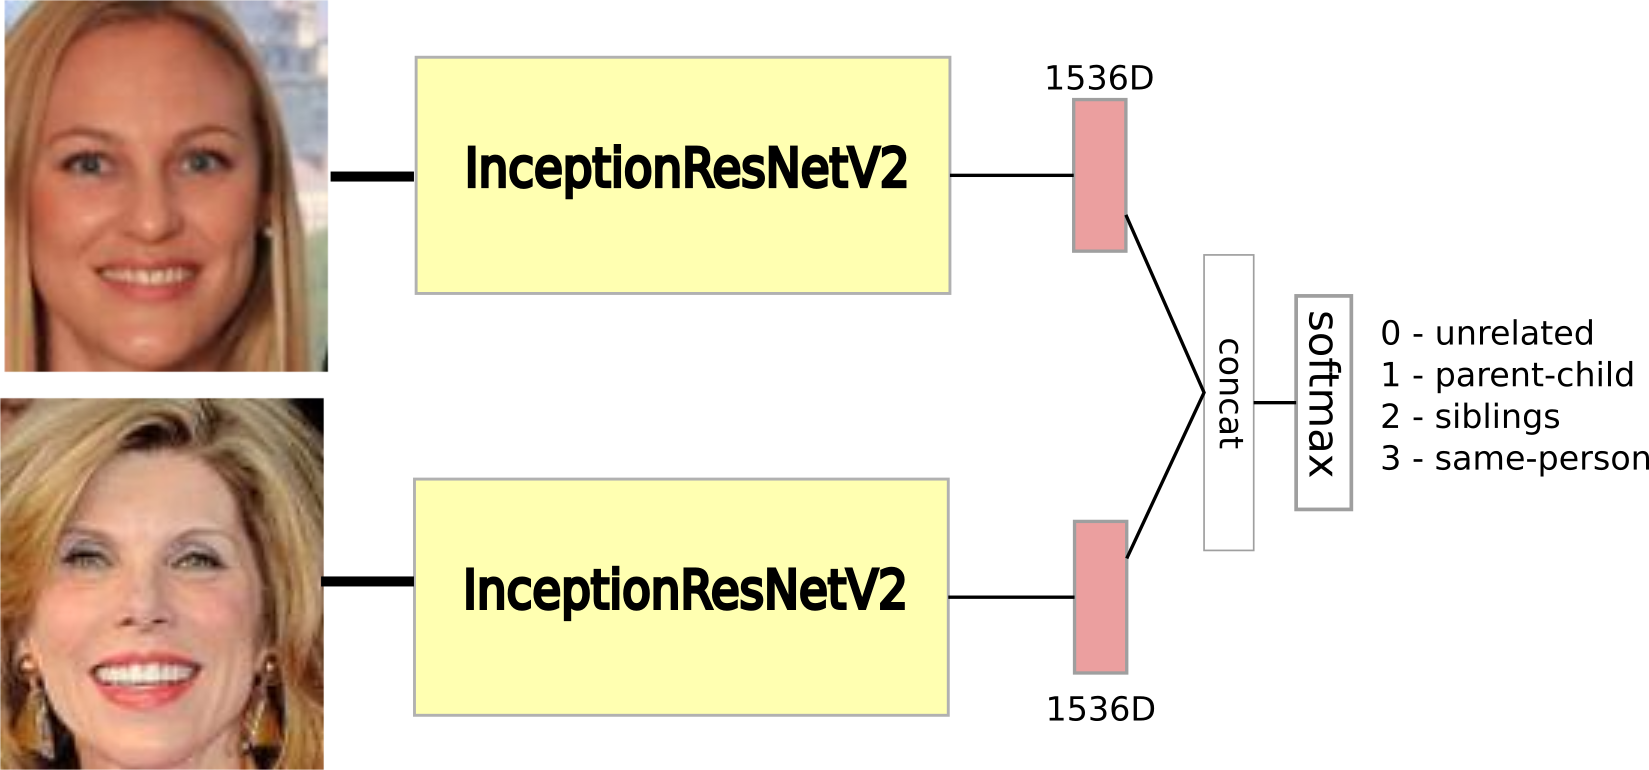
\includegraphics[width=1\textwidth]{img/model_pic1}
\end{figure}

One of the best facenet implementation models is InceptionResNetv2[11], which
possibly have a better performance than VGG-Face net. However it is very
expensive to train as it contains over 1 million parameters. Face kinship and
face recogintion are very similar problems. I am going to take pretrained
model, fitting it my new model, retain them. This could speed up the trainning
process.

Due to the original dataset uneven, training dataset are dividen into 6000
images as a test set, leaving the rest of the data as training. Both train set
and test set have equal number of image pair for each label, allowing the model
to learn evenly. Even we forsake some data volunterily, it is enought to train
the model.

In the first model, I took the InceptionResNetV2 model, removing the last full
connection layer and add global average last layer with 1536 dimension output,
following two dense layer with 1024, 128 units seperately. The finally layer is
a 4 node softmax output. For each face pair, I feed them into InceptionResNet
and get two 1536 vector which are concatenated into 3072 vector. This will feed
into dense layers to produce 4 output. Table 2 show detail architecture.

\begin{table}[h]
	\centering
	\begin{tabular}{ | l | c | c | c | c |}
		layer&size-in&size-out&param&FLPS\\
		\hline
			Input1 & 299x299x3 & & 0 & \\
			Input2 & 299x299x3 & & 0 & \\
			InceptionResNetV2 & 299x299x3 & 1x1536 & & \\
			InceptionResNetV2 & 299x299x3 & 1x1536 & & \\
			concat & 2x1536 & 1x3072 & & 0 \\
			fc1 & 1x3072 & 1x1024 & 3M & 3M \\
			fc2 & 1x1024 & 1x128 & 131K & 131K \\
			softmax & 1x1024 & 1x4 & 4100 & 4100 \\
		\hline
	\end{tabular}
	\caption{KinNet Layers}
	\label{table:2}
\end{table}

After serveral epochs of training, It started to converge, the best result we
get with 0.677 accuracy, with 1.580017 lost. It trained continuely over a
serveral days. Due to computer memory limitation, it is impossible to fit all
training image. We choose to split train set to 5000 images for each training
session, in over 5 session. It starts to overfit, training accuracy up to 98\%
but test set about 68\%.

After talking with TA who suggests to remove all the full-connected layer,
leaving only softmax layer, I started to train the second model with only
softmax layers. Due to model changes, it is not possible to reuse pretrained
weights of model I. The model is trained from imagenet model, and the accuracy
and loss improve grandually from  25\% to 45\%. After the first 8 epochs, its
test accuracy and loss won't increase any more although the training accuracy
is approaching nearly 99\%. I realize something wrong which TAs pointed me the
correct direction, to look at whether your data shuffle well. I found the
parent-child and silbing list from FIW are sorted by family id, which would
make the model learn well on training subset of families, but not on testing
families. Reshuffling the dataset indeed helps the model gain better
performance on test set.  The accuracy on test set keeps growing until 65\%
after 6 epochs. It suddenly stopped improving on test set except improving on
training set. I chose to reduce learning rate from 0.01 to 0.001, and with
lower learning rate the model resumes to its performance on test set.

\begin{table}[h]
	\centering
	\begin{tabular}{ | l | c | c | c | c |}
		layer&size-in&size-out&param&FLPS\\
		\hline
			Input1 & 299x299x3 & & 0 & \\
			Input2 & 299x299x3 & & 0 & \\
			InceptionResNetV2 & 299x299x3 & 1x1536 & & \\
			InceptionResNetV2 & 299x299x3 & 1x1536 & & \\
			concat & 2x1536 & 1x3072 & & 0 \\
			softmax & 1x1024 & 1x4 & 4100 & 4100 \\
		\hline
	\end{tabular}
	\caption{KinNet Layers Model II}
	\label{table:3}
\end{table}


github repository: https://github.com/brucelau-github/cs230

\newpage
\section*{References}
\medskip
\small
[1] Robinson, Joseph P., et al. Families in the Wild (FIW): Large-Scale Kinship
Image Database and Benchmarks. {\it Proceedings of the 2016 ACM on Multimedia
Conference} - MM '16, 2016, doi:10.1145/2964284.2967219.

[2] Schroff, F., Kalenichenko, D., \& Philbin, J. (2015). FaceNet: A unified
embedding for face recognition and clustering. {\it 2015 IEEE Conference on
Computer Vision and Pattern Recognition (CVPR)}. doi: 10.1109/cvpr.2015.7298682

[3] Wang, S., Robinson, J. P., \& Fu, Y. (2017, May). Kinship verification on
families in the wild with marginalized denoising metric learning. {\it In 2017 12th
IEEE International Conference on Automatic Face \& Gesture Recognition (FG 2017)
(pp. 216-221). IEEE}.

[4] Szegedy, C., Ioffe, S., Vanhoucke, V., \& Alemi, A. A. (2017, February).
Inception-v4, inception-resnet and the impact of residual connections on
learning. In {\it Thirty-first AAAI conference on artificial intelligence}.

[5] Deng, J., Dong, W., Socher, R., Li, L.-J., Li, K.,\& Fei-Fei, L. (2009).
ImageNet: A large-scale hierarchical image database. In {\it 2009 IEEE
conference on computer vision and pattern recognition} (pp. 248-255).

[6] Krizhevsky, Alex., Sutskever, I., \& Hinton, G. E. (2012). Imagenet
classification with deep convolutional neural networks. In {\it Advances in
neural information processing system} (pp. 1097-1105).

[7] Szegedy, c., Liu, W., Jia, Y., Sermanet, P., Reed, S., Anguelov, D., ... \& Rabinovich, A. (2015). Going deeper with convolutions. In {\it Proceedings of the IEEE conference on computer vision and pattern recognition} (pp. 1-9)

[8] Simonyan, K., \& Zisserman, A. (2014). Very deep convolutional networks for large-scale image reognition. {\it arXiv preprint arXiv}: 1409. 1556.

[9] He, K., Zhang, X., Ren, S., \& Sun, J. (2016). Deep residual learning for image recognition. In {\it Proceedings of the IEEE conference on computer vision and pateern recognition} (pp. 770-778).

[10] Huang, G. B., Ramesh, M., Berg T., \& Learned-Miller, E. (2007) Labeled faces in the wild: a database for studying face recognition in unconstraned environments. In {\it Technical Report} 07-49, October 2017

[11] Szegedy, C., Ioffe, S., Vanhoucke, V., \& Alemi, A. A. (2017, February). Inception-v4, inception-resnet and the impact of residual connections on learning. In {\it Thirty-first AAAI conference on artificial intelligence}.

\end{document}
